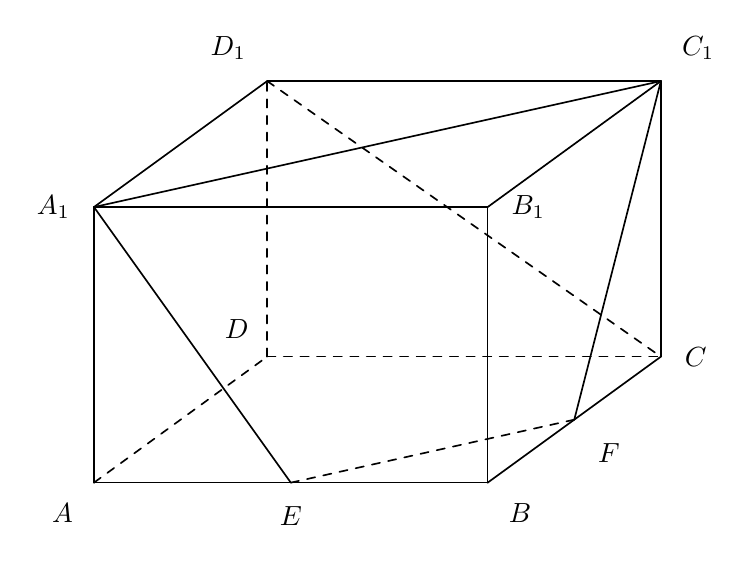
\begin{tikzpicture}[line width=0.6pt, line join=round, line cap=round]
% cuboid oblique projection, front face A-B-B1-A1
\coordinate (A) at (0,0);
\coordinate (E) at (2.5,0);
\coordinate (B) at (5,0);
\coordinate (D) at (2.2,1.6);
\coordinate (C) at (7.2,1.6);
\coordinate (F) at (6.1,0.8);
\coordinate (A1) at (0,3.5);
\coordinate (B1) at (5,3.5);
\coordinate (D1) at (2.2,5.1);
\coordinate (C1) at (7.2,5.1);
% solid cuboid edges
\draw (A) -- (B);
\draw (B) -- (C);
\draw (C) -- (C1);
\draw (C1) -- (D1);
\draw (D1) -- (A1);
\draw (A1) -- (B1);
\draw (B1) -- (C1);
\draw (A) -- (A1);
\draw (B) -- (B1);
% interior / problem lines (solid)
\draw (A1) -- (E);
\draw (A1) -- (C1);
\draw (C1) -- (F);
% hidden edges (dashed)
\draw[dashed] (A) -- (D);
\draw[dashed] (D) -- (C);
\draw[dashed] (D) -- (D1);
\draw[dashed] (D1) -- (C);
\draw[dashed] (E) -- (F);
% vertices dots (small, gray)
% labels with clearance (no touching strokes)
\node[below left=4pt] at (A) {$A$};
\node[below=5pt] at (E) {$E$};
\node[below right=4pt] at (B) {$B$};
\node[left=5pt,above=1pt,xshift=-6pt,yshift=2pt] at (D) {$D$};
\node[right=5pt] at (C) {$C$};
\node[below right=5pt] at (F) {$F$};
\node[left=5pt] at (A1) {$A_{1}$};
\node[right=5pt] at (B1) {$B_{1}$};
\node[above left=4pt] at (D1) {$D_{1}$};
\node[above right=4pt] at (C1) {$C_{1}$};
\end{tikzpicture}
